\documentclass[11pt]{scrartcl}
\usepackage[margin=2cm]{geometry}
\usepackage{amsmath}
\usepackage{amsfonts}
\usepackage{amssymb,amsmath,amsthm}
\usepackage{xcolor} 
\usepackage{enumitem}
\usepackage{tikz} 
\usepackage{float}
\usepackage{color}
\definecolor{myblue}{rgb}{.8, .8, 1}
\usetikzlibrary{shapes.geometric,calc}
\addtokomafont{section}{\rmfamily\centering\scshape}
% math environments 
\usepackage[utf8]{inputenc}
\theoremstyle{definition}
\newtheorem{theorem}{Theorem}
\newtheorem{corollary}{Corollary}
\newtheorem{lemma}[theorem]{Lemma}
\newtheorem{definition}{Definition}
\newtheorem{prop}{Proposition}
\newtheorem{ex}{Example}
\theoremstyle{remark}
\newtheorem{remark}{Remark}
% boxes
\usepackage{empheq}

\newlength\mytemplen
\newsavebox\mytempbox

\makeatletter
\newcommand\mybluebox{%
    \@ifnextchar[%]
       {\@mybluebox}%
       {\@mybluebox[0pt]}}

\def\@mybluebox[#1]{%
    \@ifnextchar[%]
       {\@@mybluebox[#1]}%
       {\@@mybluebox[#1][0pt]}}

\def\@@mybluebox[#1][#2]#3{
    \sbox\mytempbox{#3}%
    \mytemplen\ht\mytempbox
    \advance\mytemplen #1\relax
    \ht\mytempbox\mytemplen
    \mytemplen\dp\mytempbox
    \advance\mytemplen #2\relax
    \dp\mytempbox\mytemplen
    \colorbox{myblue}{\hspace{1em}\usebox{\mytempbox}\hspace{1em}}}

\makeatother


% definition
\newcommand{\dfn}[1]{\textbf{\underline{#1}}}
\newcommand{\dist}[0]{\mathcal{F}}
\newcommand{\pr}[1]{\mathbb{P}[#1]} 
\newcommand{\stat}[0]{T(X_1, ..., X_n )} 

% converge in probability 
\newcommand{\cvp}[0]{\overset{p}{\to}}

% sample mean
\newcommand{\smean}[0]{\frac{1}{n} \sum_{i=1}^n x_i} 

% sample variance
\newcommand{\svar}[0]{\frac{1}{(n-1)} \sum_{i=1}^n (x_i - \overline{x})^2}

% expected value 
\newcommand{\EX}[1]{\mathbb{E}\left[#1 \right]}  
\newcommand{\EXth}[1]{\mathbb{E}_\theta \left[ #1 \right]}

% integral
\newcommand{\idx}[2]{\int_{#1}^{#2}}

% vector
\newcommand{\vect}[1]{\mathbf{#1}}

% symbols
\newcommand{\R}[0]{\mathbb{R}}


\title{\textbf{Math 475: Partial Differential Equations}}
\author{Shereen Elaidi}
\date{Fall 2019 Term}

\begin{document}

\maketitle
\tableofcontents

\section{Introduction}

\textbf{Q:} Where do PDE's come from? PDEs are used in all types of math modelling; they translate phenomena coming from physics, biology, chemistry, etc. into mathematical terms. 
\newline 
\newline 
\textbf{Q:} What goes into a PDE model? 
\begin{center}
	Math model = General Physical Laws (balancing forces and conservation of quantities) + Constitutive Relations (Laws specific to the environment, e.g. Fick's Law of Diffusion) 
\end{center}
A PDE $\leftrightarrow$ a physical description of a system. 

\begin{definition}[PDE]
	A \dfn{PDE} is a mathematical relation involving partial derivatives, i.e., if $\vect{u}: \R^n \rightarrow \R$, $\vect{x} = (x_1, ..., x_n)$ a real-valued function of several variables, then any kth order PDE can be expressed as: 
	\begin{align}
		F(D^k \vect{u}, D^{k-1} \vect{u}, ..., D \vect{u}, \vect{u}, \vect{x} ) = 0 \text{ in } \Omega 	
	\end{align}
	where $\Omega \subseteq \R^n$ is the domain or region where the PDE holds, and $F$ is a function of the placeholders. 
\end{definition}

\begin{definition}[$C^k$ and $C^k(\Omega)$] A function $\vect{u}: \R^n \rightarrow \R$ is $C^k$ at a point $\vect{x} \in \R^n$ if every kth-order partial derivative is continuous as a function of $\R^n$ at $x$. If $u \in C^2(\R^n)$, then in advanced calculus it was proven that $D^2u$ is a symmetric matrix. 
\end{definition}

\begin{ex}[Examples of PDEs] 
	\begin{enumerate}[noitemsep]
		\item \dfn{Heat Equation}: 
		\begin{align}
				u_t - k \Delta u = u_t - k \sum_{i=1}^n u_{x_i x_i} = 0 
		\end{align}
		where $k > 0$ is a constant. Then the solution has a space- and time- component: 
		\begin{align}
			u(\vect{x}, t) = u: \R^{n+1} \rightarrow \R 
		\end{align}
	\item \dfn{Laplace's Equation}: 
	\begin{align}
			- \Delta u = 0 
	\end{align}
	$u(x)$ is the steady state of a solution to the heat equation, since $u_t = 0 \Rightarrow$ ``constant in time.'' The solution $u$ is a function $u: \R^n \rightarrow \R$. 
	\item \dfn{Wave Equation}: 
	\begin{align*}
		& u_{tt} - \Delta u = 0 \\
		& u: \R^{n+1} \rightarrow \R 
	\end{align*}
	$u(x,t)$ is the displacement of an object with wave-like behaviour at location $\vect{x}$ and time $t$. Ex: position of a guitar string. 
	\item \dfn{Transport Equation}: 
	\begin{align*} 
		u_t + cu_x = 0,\ c \in \R, u: \R^2 \rightarrow \R \text{ (space, time) } 
	\end{align*} 
	$u(x,t)$ can be the density of a pollutant at location $\vect{x}$ and time $t$. 
	\item  \dfn{Reaction-Diffusion}: 
	\begin{align*}
		& u_t - k \Delta u = f(u) \\
		& u: \R^{n+1} \rightarrow \R \\
		& f: \R \rightarrow \R 	
	\end{align*}
	$u( \vect{x},t)$ can be the temperature at location $(\vect{x}, t)$ subject to enhancement by $f(u)$ (for example, fire spreading). 
	\item \dfn{Burger's Equation}: 
	\begin{align}
		u_t - u u_x = vu_{xx} 
	\end{align}
	$v > 0$ represents the viscosity. $u: \R^2 \rightarrow \R$, $u(x,t)$ is the concentration of a material in a fluid flow with convection. 
	\end{enumerate}	
\end{ex}

\subsection{Domains and Boundary Conditions}

\begin{definition}[$C^1$ domain] 
	$\Omega \subseteq \R^n$ is a \dfn{$C^1$ domain} if $\partial \Omega$ can locally be expressed as a graph of a $C^1$ function. This means...
	\begin{enumerate}[noitemsep]
		\item $\partial \Omega$ has no corners $\Rightarrow$ smooth. 
		\item $\forall p \in \partial \Omega$, there exists a well-defined and unique tangent plane (whose slope is given by the derivative), which implies that there exists a well-defined inward and outward normal vector. 
		\item Inward and outward normal vectors move continuously along $\partial \Omega$. 
	\end{enumerate}
\end{definition}

\subsubsection{What are the main boundary conditions?}
\begin{enumerate}[noitemsep]
	\item \dfn{Dirichlet Boundary Conditions}: these prescribe what $u$ is on $\partial \Omega$. We assume that $u \in C^k(\Omega) \cap C(\partial \Omega)$. 
	\item \dfn{Neumann Boundary Conditions}: these prescribe what the normal derivative of $u$ on $\partial \Omega$ is. The meaning behind this is: \emph{how does $u$ change along the boundary}? It is specifying:
	\begin{align}
		\frac{\partial u}{\partial n} = \nabla u \cdot n(x) = X \text{ on } \partial \Omega 	
	\end{align}
	\item \dfn{Robin boundary conditions}: a combination of the above: 
	\begin{align}
		\frac{\partial u}{\partial n} + \alpha u = X \text{ on } \partial \Omega 
	\end{align}
\end{enumerate}
In general, in PDEs, we will not be able to identify an explicit solution. Thus, we care about the following four fundamental issues. The first three ensure that we have a \emph{well-posed problem}, and the final one is important when we cannot obtain an explicit solution. 
\begin{enumerate}[noitemsep]
	\item \emph{Existence}: is there a solution? 
	\item \emph{Uniqueness}: is there exactly one solution to the PDE?
	\item \emph{Stability}: does the solution depend continuously on the data? 
	\item \emph{Qualitative Properties}: If I cannot find an explicit solution, but I know that it exists, what else can I tell you about the solution? Some questions we are interested in studying are: 
	\begin{enumerate}[noitemsep]
		\item Does $u(\vect{x}, t) \rightarrow 0$ as $t \rightarrow \infty$? 
		\item What is $\max_\Omega |u(\vect{x})|$? 
	\end{enumerate}
\end{enumerate}

\subsection{Classification of PDEs} 
To do: draw out the chart 

When we have a PDE that's linear in $D^2u$, we can always express our PDE in the form of a matrix: 
\begin{align}
	F(D^2u, Du, u, x) = \underbrace{- \sum_{i=1}^n \sum_{j=1}^n A_{ij}(x) u_{x_ix_j}}_{:=L[u]}  + G(Du, u, x) 
\end{align}
where $A \in $ MAT$(n \times n, \R)$ is symmetric, since $u \in C^2$. $L[u]$ is a linear operator that maps functions to functions and is of the form
\begin{align}
	L[u] = -\text{tr}( A(x) D^2(u)) 	
\end{align}
Therefore, we can write linear, second-order PDEs in the following form: 
\begin{align}
	-\text{tr}(A(x) D^2 u) = G(Du, u,x) 	
\end{align}
This is useful since we can classify second-order PDEs in terms of the eigenvalues of $A$. We will now give definitions for the three main types of PDEs: 

\begin{definition}[Elliptic PDE]
	A PDE is \dfn{elliptic} if $\forall x$, $A(x)$ has non-zero eigenvalues, all of which have the same sign. 
\end{definition}

The model equation for an elliptic PDEs is: 
\begin{align}
	- \Delta u = -\sum_{i=1}^n u_{x_i x_i} = - \sum_{i,j =1}^n A_{ij}(x) i_{x_i x_j} 	
\end{align}
where 
\begin{align}
	A(x) = \begin{bmatrix}
		1 &  &  & \\
		  & 1 & & \\
		  &  &  \ddots & \\
		  & & & 1 
	\end{bmatrix}	
\end{align}

\begin{definition}[Hyperbolic PDE]
	A PDE is \dfn{hyperbolic} if $\forall x$, $A_{ij}(x)$ has non-zero eigenvalues, all of the same sign except for one. 
\end{definition}

The model equation for a hyperbolic PDE is: 
\begin{align}
	\text{ wave equation: } u_{tt} - \Delta u = - \text{tr} (A(x,t) D_{x,t}^2 u ) 	
\end{align}
where 
\begin{align}
	A(x,t) = 	\begin{bmatrix}
		1 &  &  & \\
		  & \ddots & & \\
		  &  &  1 & \\
		  & & & -1
	\end{bmatrix}	
\end{align}

\begin{definition}[Parabolic PDE]
	A PDE is \dfn{parabolic} if $\forall x$, $A(x)$ has at least one zero eigenvalue. 
\end{definition}

The model equation for a parabolic PDE is: 
\begin{align}
	\text{ Heat Equation: } u_t - \Delta u = - \text{tr}(A_{ij}(x) D_{x,t}^2 u) + u_t 	
\end{align}
where 
\begin{align}
	A(x,t) = 	\begin{bmatrix}
		1 &  &  & \\
		  & \ddots & & \\
		  &  &  1 & \\
		  & & & 0
	\end{bmatrix}_{(n+1, n+1)}	
\end{align}

\begin{remark}
	Typically, a parabolic PDE can be written down as $u_t + $ elliptic PDE. Thus, we would expect them to have similar properties (which they do, as we will see later). 
\end{remark}
In this course, we'll focus on heat, wave, and Laplace's equations as models of parabolic, hyperbolic, and elliptic PDEs. 

\section{Diffusion}
\textbf{Physical Phenomena:} heat flow, diffusion of ink, and transport of a substance due to the molecular motion of the surrounding medium. 

\subsection{Derivation and Setting Up $(n=1)$}
Let $u(x,t)$ be the temperature at location $x \in \R$, and let $t$ be the time, $t > 0$. We're going to consider a rod of length $L$, going from $x=0$ to $x=L$. We will assume perfect insulation of the tube as well as constant mass density. This gives us a one-dimensional model, since heat is flowing in only one direction. In the rod, consider an cross section $S$.   

%\begin{center} 
%\begin{tikzpicture}
%  \node[cylinder,draw=black,thick,aspect=0.7,minimum height=12cm,minimum     width=0.7cm,shape border rotate=0,cylinder uses custom fill, cylinder body     fill=blue!30,cylinder end fill=blue!10] (A) {};
%
%\draw[dashed]
%    let \p1 = ($ (A.after bottom) - (A.before bottom) $),
%        \n1 = {0.5*veclen(\x1,\y1)-\pgflinewidth},
%        \p2 = ($ (A.bottom) - (A.after bottom)!.5!(A.before bottom) $),
%        \n2 = {veclen(\x2,\y2)-\pgflinewidth}
%  in
%    ([xshift=-\pgflinewidth] A.before bottom) arc [start angle=270, delta angle=180,
%    x radius=\n2, y radius=\n1];
%\end{tikzpicture}
%\end{center} 

Define the following quantities: 
\begin{align*}
	& e(x,t) := \text{ thermal energy / unit mass } \\
	& q(x,t) := \text{ heat flux (rate of flow per unit area) } \\
	& \rho := \text{ mass density per unit volume} \\
	& r(x,t) := \text{ rate / unit mass of the external heat source} 	\\
	& \rho(1/A) := A 
\end{align*} 
The general physical law that we will use is: 
\begin{align*}
	\text{ Rate of thermal energy change in } S =  \text{ heat in } - \text{ heat out (via the ends) }
\end{align*} 
\begin{enumerate}[noitemsep]
	\item For the rate of thermal energy change in $S$, we have that this equals the derivative with respect to dime of the thermal energy in $S$. If we let $x_0$ be the left end point of $S$ and $x_0 + \Delta x$ be the right end point of $S$, then the total thermal energy in $S$ equals
	\begin{align}
		\text{ thermal energy in } S = \int_{x_0}^{x_0 + \Delta x} e(x,t) \rho A dx := E(t) 
	\end{align}
	where $e(x,t)$ is the thermal energy per unit area, $\rho$ is the density, and $A$ is the area. Assuming that we can interchange the derivative with the limit, we obtain: 
	\begin{align}
		\frac{dE}{dt} = \idx{x_0}{x_0 + \Delta x} \frac{\partial e}{\partial t} e(x,t) \rho A dx 	
	\end{align}
	\item Now for the heat in $-$ heat out via the ends term, we need to account for both the external heat source and the heat flow through the ends. Contribution from an external heat source could be from an electric current or a chemical reaction. We will use the \dfn{law of conservation of energy}, which can be formulated as: \emph{the time rate of change of thermal energy in $S$ = the net flux through $\partial S$ due to conduction $+$ time rate at which heat is supplied by the external sources }. Therefore, the contribution from the heat source is given by: 
	\begin{align*}
		\idx{x_0}{x_0 + \Delta x} r(x,t) \rho A dx 	
	\end{align*}
	and the flux through the ends is divergence, meaning that
	\begin{align*}
		\text{flux} = -q(x,t) \cdot n
	\end{align*}
	where $n$ is the outward unit normal. Therefore, the energy flow rate through $[x, x+ \Delta x]$ is $-(q(x_0+ \Delta x, t) - q(x_0, t)) \cdot A$. If $q$ is differentiable in $x$ then by the fundamental theorem of calculus, we obtain: 
	\begin{align}
		\text{flux} = - \idx{x_0}{x_0 + \Delta x} A \frac{\partial q}{\partial x} q(x,t) dx 	
	\end{align}
	So, putting all the previous equations together, by the general physical laws we obtain: 
	\begin{align}\label{generalphyslaws}
		\idx{x_0}{x_0 + \Delta x} \frac{\partial e}{\partial t} [ e(x,t)] \rho A dx = \idx{x_0}{x_0 + \Delta x} r(x,t) \rho A dx - \idx{x_0}{x_0 + \Delta x} A \frac{\partial q}{\partial x} q(x,t) dx
	\end{align}

\end{enumerate}
The constitutive relations that we will use are the \dfn{Fourier Law of Heat Conduction} and a relationship between thermal energy and temperature. 
\begin{enumerate}[noitemsep]
	\item \dfn{Fourier Law of Heat Conduction}: Heat flux is a linear combination of the temperature gradient heat flows from hot to cold. For $\kappa >0$ a constant, this is expressed as: 
	\begin{align}
		q(x,t) = - \kappa u_x	
	\end{align}
	(If the temperature is decreasing with respect to space, then heat is flowing out and the flow is positive). 
	\item For thermal energy, we have that it is a linear function of the absolute temperature. Let $c > 0$ be the specific heat. Then: 
	\begin{align}
		e(x,t) = cu(x,t) 
	\end{align}
	Which implies that
	\begin{align*}
		\frac{\partial e}{\partial t} = cu_t \text{ and } \frac{\partial q}{\partial x} = - \kappa u_{xx} 	
	\end{align*}
\end{enumerate}
	Substituting these constitutive relations into (\ref{generalphyslaws}), we obtain: 
\begin{align*}
	 & \idx{x_0}{x_0 + x} cu_t \rho dx = \idx{x_0}{x_0 + x}  r(x,t) \rho dx - \idx{x_0}{x_0 + x}  - \kappa u_{xx} dx \\
	\iff & \idx{x_0}{x_0 + x}  ( c \rho u_t - \kappa u_{xx} ) dx = \idx{x_0}{x_0 + x}  \rho r(x,t) dx \\
	\iff & \idx{x_0}{x_0 + x}  \left[ u_t - \frac{\kappa}{c \rho} u_{xx} \right] dx = \idx{x_0}{x_0 + x}  \frac{1}{c} r(x,t) dx 
\end{align*}
Since $]x_0, x_0 + \Delta x[$ is an arbitrary interval, equality of the integrals $\Rightarrow$ equality of the functions holds pointwise: 
\begin{align*}
	u_t - \frac{\kappa}{c \rho} u_{xx} = \frac{1}{c} r(x,t) 
\end{align*}
where $k := \kappa / cp$ is called the \dfn{diffusion constant.} If there is no external heat source, then the diffusion equation in one-dimension is given by: 
\begin{empheq}[box={\mybluebox[5pt]}]{equation}
    u_t - ku_{xx} = 0 
\end{empheq}
and if there is a heat source, i.e., $r(x,t) \neq 0$, then: 
\begin{empheq}[box={\mybluebox[5pt]}]{equation}
    u_t - ku_{xx} = \tilde{r}(x,t) 
\end{empheq}
$k$ encodes the thermal response time of the material. Now, we want to study the temperature in the rod by starting with an initial temperature distribution $u(x,0) := g(x)$. Boundary conditions would be of the form: 
\begin{itemize}[noitemsep]
	\item \dfn{Dirichlet Boundary Conditions}: $u(0,t) = h_1(t)$ and $u(L,t) = h_2(t)$. 
	\item \dfn{Neumann Boundary Conditions}: prescribe a heat flux at the ends: 
	\begin{align*}
		& u_x(0,t) = h_1(t) \\
		& u_x(L,t) = h_2(t) 
	\end{align*}
	\item \dfn{Robin Boundary Conditions}: heat flux on the ends is proportional to the difference between the temperature and its surroundings. In this case, we have an equation of the form: 
	\begin{align*}
		k u_x = \gamma (U-u) 
	\end{align*}
	where $\gamma > 0$ and $U$ is the temperature of the surroundings. 
	\begin{align*}
		& \Rightarrow u_x + \frac{\gamma }{k} u = \frac{\gamma'}{k} U \\
		& \Rightarrow u_x(0,t) + \alpha u(0,t) = h_1(t) \\
		& \Rightarrow u_x(L,t) + \alpha u(L, t) = h_2(t) 
	\end{align*}
	i.e., we have a linear combination of dirichlet and Neumann boundary conditions. 
\end{itemize}
If $h_1 = h_2 = 0$ then we have \dfn{homogeneous boundary conditions}. 

\subsubsection{Boundary Value Problems in $L_T:= ]0, L[ \times ]0, T]$}
Let $\partial p L_T :=$ the parabolic boundary of $L_T$. It is the union of the initial data (blue) and the boundary data (yellow) of the figure below. 
\begin{figure}[H]
	\centering 
	\label{parabolicbdry}
	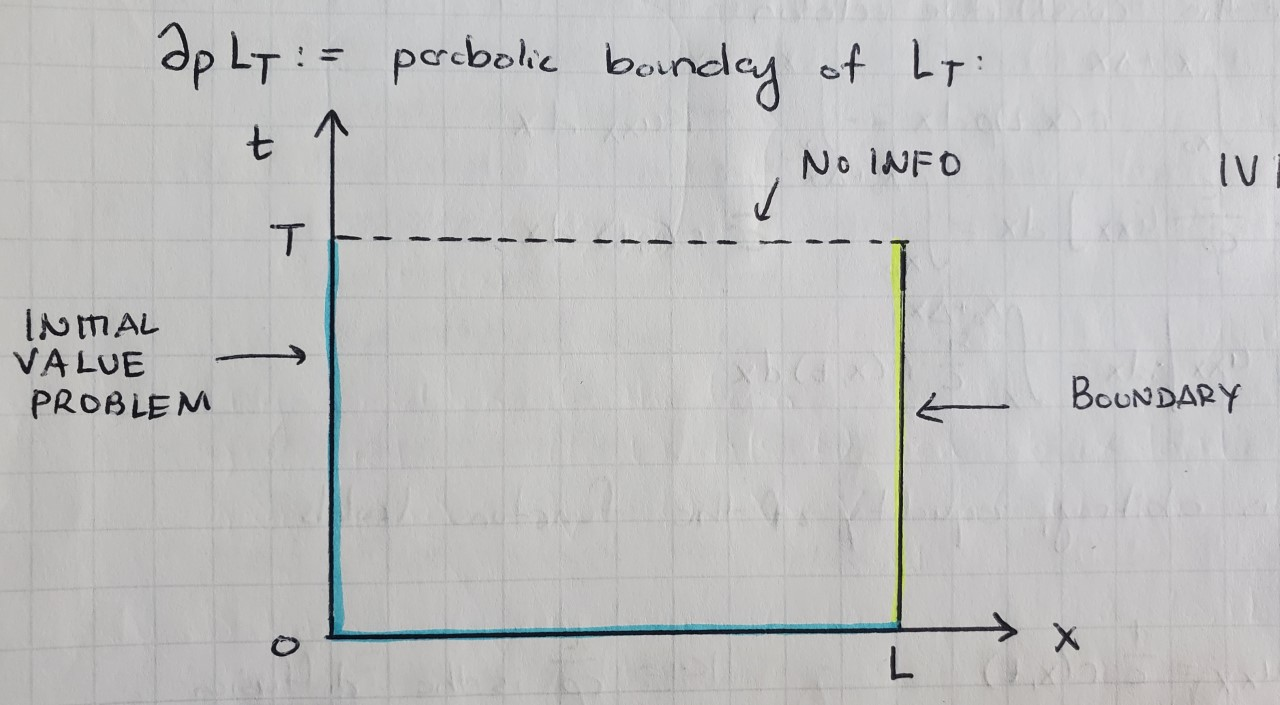
\includegraphics[width=10cm]{pbdry}
\end{figure}
We require that $u \in C^{(2,1)}(L_T) \cap (\partial p L_T)$ (we have $C^{(2,1)}$ for two spatial dimensions and one time-dimension. The two main types of questions in this chapter are: 
\begin{align*}
& \text{ Boundary Value Problem:  } 
\begin{cases}
	 u_t - ku_{xx}  = r(x,t) & \text{ in } L_T \\
	 u(x,0) = g(x) & \text{ in } [0,L] \\
	 + \text{ B.C. } \\
\end{cases}	
\\
& \text{ Global Cauchy Problem: } \begin{cases}
	 u_t - ku_{xx}  = r(x,t) & \text{ in } \R \times ]0, T] \\
	 u(x,0) = g(x) & \text{ in } \R \\
	 + \text{ conditions on $u$ as } x \rightarrow \pm \infty  \\
\end{cases}
\end{align*}

\subsection{Derivation in $n \geq 1$}
The law of conservation of energy can be formulated as
\begin{center}
	Rate of Change of Heat Energy in a volume $V$ = Net Heat Flow Through $\partial V$
\end{center}
Again, define
\begin{align*}
	& e(x,t) := \text{ thermal energy / unit mass} \\
	& q(x,t) := \text{ heat flux (vector) } \\
	& \rho := \text{ mass density / unit volume} 
\end{align*}
Using the same constitutive relations as before and applying the divergence theorem, we obtain:
\begin{align*}
	\idx{V}{} \frac{\partial e}{\partial t} e(x,t) \rho dx & = \idx{V}{} r(x,t) \rho dx - \idx{\partial V}{} q(x,t) \cdot v d \sigma \\
	& = \idx{V}{} r(x,t) \rho dx - \idx{V}{} \text{div}(q(x,t)) dx 
\end{align*}
By the same constitutive relations, 
\begin{align*}
	& e(x,t) = cu(x,t) \\
	& q(x,t) = - \kappa \nabla u \\
	& \text{div}(\nabla u) = \Delta u
\end{align*}
Which gives us that
\begin{align*}
	\idx{V}{} c u_t \rho dx = \idx{V}{} r(x,t) \rho dx + \idx{V}{} \kappa \Delta u dx 
\end{align*}
Pointwise equality follows from the fact that $V \subseteq \R^n$ is arbitrary, and so
\begin{align*}
	& c u_t \rho = r(x,t)\rho + k \Delta u \\
	\iff & u_t - k \Delta u = \tilde{r}(x,t) \text{ in } \R^n \times ]0, \infty [
\end{align*}


\end{document}